%%%%%%%%%%%%%%%%%%%%%%%%%%%%%%
% LATEX-TEMPLATE TECHNISCH RAPPORT
%-------------------------------------------------------------------------------
% Voor informatie over het technisch rapport, zie
% http://practicumav.nl/onderzoeken/rapport.html
% Voor readme en meest recente versie van het template, zie
% https://gitlab-fnwi.uva.nl/informatica/LaTeX-template.git
%%%%%%%%%%%%%%%%%%%%%%%%%%%%%%

%-------------------------------------------------------------------------------
%	PACKAGES EN DOCUMENT CONFIGURATIE
%-------------------------------------------------------------------------------

\documentclass{uva-inf-article}
\usepackage[dutch]{babel}
\usepackage[utf8]{inputenc}
\usepackage{hyperref}
\usepackage{csquotes}
\usepackage{graphicx} 
\usepackage{listings}
\graphicspath{ {./images/} }

% Relevant voor refereren vanaf blok 5
%\usepackage[style=authoryear-comp]{biblatex}
%\addbibresource{bib}

%-------------------------------------------------------------------------------
%	GEGEVENS VOOR IN DE TITEL
%-------------------------------------------------------------------------------

% Vul de naam van de opdracht in.
\assignment{ Data Analyse en Visualisatie}
% Vul het soort opdracht in.
\assignmenttype{Technisch Rapport}
% Vul de titel van de eindopdracht in.
\title{Universities got talent: Hoe verdient een universiteit zijn score?}

% Vul de volledige namen van alle auteurs in.
\authors{Kalle Janssen; Wijnand Potthoff; Daniel Jensen Perez; Anthony Thieme;}
% Vul de corresponderende UvAnetID's in.
\uvanetids{11882107; 10780726; 11610964; 11872934}

% Vul altijd de naam in van diegene die het nakijkt, tutor of docent.
\tutor{Mattijs Blankesteijn}
% Vul eventueel ook de naam van de docent of vakcoordinator toe.
\docent{}
% Vul hier de naam van de PAV-groep  in.
\group{Naam van de groep}
% Vul de naam van de cursus in.
\course{Data Analyse en Visualisatie}
% Te vinden op onder andere Datanose.
\courseid{5082DAAV6Y}

% Dit is de datum die op het document komt te staan. Standaard is dat vandaag.
\date{\today}

%-------------------------------------------------------------------------------
%	VOORPAGINA
%-------------------------------------------------------------------------------

\begin{document}
\maketitle

%-------------------------------------------------------------------------------
%	INHOUDSOPGAVE EN ABSTRACT
%-------------------------------------------------------------------------------

% Niet doen bij korte verslagen en rapporten
%\tableofcontents
%\begin{abstract}
%\lipsum[13]
%\end{abstract}

%-------------------------------------------------------------------------------
%	INTRODUCTIE
%-------------------------------------------------------------------------------

\section*{Introductie}

Iedereen kent ze wel, the university of Oxford, the university of Cambridge, MIT en Harvard. Deze universiteiten behoren tot de beste universiteiten van de wereld. Waarom zijn deze universiteiten zo goed? Wat is het verschil met andere universiteiten? Er zijn veel aspecten waarop een universiteit in kwaliteit beoordeeld kan worden. Ook is het zo dat niet alles directe invloed heeft op het niveau van de opleidingen die een instituut aanbied.

In dit onderzoek zal er worden gekeken naar de invloed van de scores van verscheidene aspecten op de uiteindelijke ranking van een universiteit. Deze scores zijn verkregen van de Times Higher Education World University Ranking \cite{Times}, van de jaren 2016, 2016 en 2018. Deze rangijst maakt gebruik van tien verschillende factoren om een zo uitgebreid mogelijk beeld te kunnen geven van de status van 's werelds top universiteiten, en wordt dan ook gerespecteerd door studenten, academici en overheden. De vraag is of er specifieke factoren zijn die een sterke invloed uitoefenen op de uiteindelijke kwaliteit van een universiteit. Door middel van diepgaande data-analyse zal er vanuit de verkregen scores naar opvallende verbanden worden gezocht vanuit grafische weergaven van de dataset.


Ook zal er worden gezocht naar de meest consistente en inconsistente universiteiten en regio's binnen deze ranglijst. Daarnaast zal er ook naar de meest opvallende en relevante verschillen in de top tweehonderd universiteiten worden gezocht, en uiteindelijk of er zich andere interessante patronen voordoen binnen de dataset. Hiervoor zal deze vergeleken worden met een dataset betreffende het bruto nationaal product van de landen waarin de gerankte universiteiten zich bevinden.

In dit onderzoek wordt uitgegaan van de hypothese dat er een of meerdere factoren bestaan die een directe invloed uitoefenen op de ontvangen score van een universiteit. Er wordt verwacht vanuit de subscores van de universiteiten een duidelijke correlatie te kunnen vinden met de algemene score en rang van een universiteit. Een andere verwachting is een trend in de compositie van studenten aan een universiteit en de score, namelijk dat een hoger scorende universiteit een groot percentage aan internationale studenten zal hebben, en een vergelijkbare hoeveelheid aan mannelijke en vrouwelijke studenten bevat.

%-------------------------------------------------------------------------------
%	METHODE
%-------------------------------------------------------------------------------

\section*{Methode}

De data die gebruikt is in dit onderzoek is verkregen van de website van de Times Higher Education World University Rankings \cite{Times}. Op deze website wordt er vanaf 2011 elk jaar  een ranglijst bij gehouden met 's werelds top universiteiten. Voor dit onderzoek is er alleen gekeken naar de top achthonderd rannglijsten uit de jaren 2016, 2017 en 2018. Er is voor de top achthonderd gekozen omdat er in de ranglijst uit het jaar 2016 maar 800 universiteiten stonden. In de jaren 2017 en 2018 waren dit er veel meer. Om de jaren zo goed mogelijk te vergelijken wordt er dus alleen naar de top achthonderd gekeken. Deze dataset bevat tien verschillende factoren die een universiteit zijn ranking geven. Er wordt informatie gegeven betreffende studenten, namelijk de hoeveelheid studenten, de hoeveelheid studenten per staflid, het percentage internationale studenten en de verdeling tussen mannelijke en vrouwelijke studenten. Daarnaast worden er in de dataset de scores van verschillende aspecten van de universiteiten weergegeven, hetgeen zijn de algemene score, de \textit{teaching} score, de \textit{research} score, de \textit{citations} score, de \textit{industry income} score en de score van de \textit{international outlook}.

Voor het scrapen van de data werd er gebruik gemaakt van de Python requests package. Het opgevraagde HTML-bestand bevatte echter niet de benodigde tabel, aangezien deze interactief door JavaScript werd geladen. Er is vervolgens een webdriver gebruikt om de tabel uit te lezen en zo de relevante data te scrapen. 

Omdat er veel data-punten misten in de kolommen \textit{score\_industry} \textit{ pct\_intl\_student, male/female ratio en score\_overall} is er naar een manier gezocht om deze in te vullen. Uiteindelijk werd er gekozen om de missende data-punten in de kolommen \textit{score\_industry en score\_overall} in te vullen door middel van machine learning. Hiervoor werd de python module scikit-learn [referentie naar scikit-learn] gebruikt. De data-punten werden ingevuld door middel van \textit{multiple} lineaire regressie. Dit is een vorm van machine learning die geleend is van statistiek. Om de \textit{classifier} te trainen zijn alle rijen in de data-set gebruikt die geen data-punten misten in de kolommen \textit{ranking, score\_overall, score\_teaching, score\_research, score\_citation en score\_int\_outlook}. Deze kolommen waren de \textit{features} voor de classifier, met de \textit{features} kan  getracht worden de waarde van een gekozen \textit{label} te voorspellen. Deze classifier werd vervolgens gebruikt om alle rijen waarin er missende waarden waren voor de kolommen score\_overall en score\_industry in te vullen. Dit deed hij met een nauwkeurigheid van 99.9\% en 52\% respectievelijk. De \textit{male/female ratio} bleek slechts 15 procent accuraat, en de verkregen data is dan ook niet gebruikt. Voor deze kolom is uiteindelijk de gemiddelde man/vrouw verdeling van alle universiteiten per land genomen voor elke universiteit waar deze data miste.

De manier waarop de \textit{classifier} getraind werd hetzelfde voor \textit{score\_overall} en \textit{score\_industry}. Alle kolommen die geen datapunten misten werden apart gehouden en opgesplitst in \textit{training} en \textit{testing} data. 75\% en 25\% respectievelijk. De training data werd gebruikt om de classifier te trainen en de testing data om te berekenen in hoeveel procent van de gevallen de \textit{classifier} het goed had[citatie code op github maybe? github.com/danielperezjensen/bscKI-data-analyse/preprocessing/fill.py]. De getrainde \textit{classifier} werd vervolgens door elke rij met missende data gehaald om alle missende datapunten in te vullen.

Om een duidelijke weergave van de verbanden binnen de dataset te kunnen bieden, is er de keuze gemaakt om deze in meerdere grafische voorstellingen te verwerken met behulp van \textit{Bokeh}\cite{Bokeh}. \textit{Bokeh} is een interactieve visualisatie-bibliotheek die zich richt op moderne webbrowsers voor presentaties met als doel het bieden van elegante veelzijdige grafische voorstellingen.
Er zijn met \textit{Bokeh} een aantal plots gemaakt.Er zijn staafdiagrammen van het aantal universiteiten per continent, voor alle drie de jaren, gemaakt om de consistentie van de universiteiten binnen deze gebieden weer te geven. Een staafdiagram van de universiteiten per regio werden toegevoegd voor een specifiekere blik. Om een mogelijk verband in de top tweehonderd universiteiten aan te tonen is een tornadodiagram gemaakt van de verdeling tussen de mannen en vrouwen die aan deze universiteiten studeerden, en een scatterplot voor het percentage intenationale studenten per universiteit. Voor eventuele andere verband zijn er een histogram met de verdeling van de scores per universiteit gemaakt, evenals een radar plot betreffende het percentage internationale studenten, het percentage mannelijke studenten, de hoeveelheid studenten en het percentage staf per student. 

Voor het maken van een interactieve wereldkaart die het aantal gerankte universiteiten per land weergeeft is geen gebruik gemaakt van \textit{Bokeh}, maar in plaats daarvan gekozen voor \textit{Plotly}\cite{Plotly}. \textit{Plotly} is net als \textit{bokeh} een interactieve visualisatie-bibliotheek die zich richt op moderne webbrowsers voor presentaties, maar het maken van een wereldkaart was hiermee aanzienlijk eenvoudiger.

Om dit duidelijk online weer te kunnen geven, is er op de aangewezen server de mogelijkheid gecreëerd om de informatie per werelddeel per jaar weer te kunnen geven. 

Daarnaast wordt er ook nog gekeken of een hoog Bruto Nationaal Product (BNP oftwel GDP) een positieve invloed heeft op de gemiddelde scores en ranking van universiteiten van een land. Hiervoor wordt extra dataset gebruikt van de \textit{Cental Intelligence Agency} \cite{CIA} die het GDP weergeeft.
Om dit te kunnen vergelijken moet voor elk land de gemiddelde ranking en de gemiddelde scores berekend worden en vervolgens vergeleken worden met het GDP van het betreffende land.


%-------------------------------------------------------------------------------
%	RESULTATEN
%-------------------------------------------------------------------------------

\section*{Resultaten}
Alle resultaten betreffende studenten en universiteiten zijn naar beneden afgerond.

Voor het vinden van de constistentie van de scores van universiteiten per regio is de volgende plot gecreëerd.\\
\begin{figure}[h]
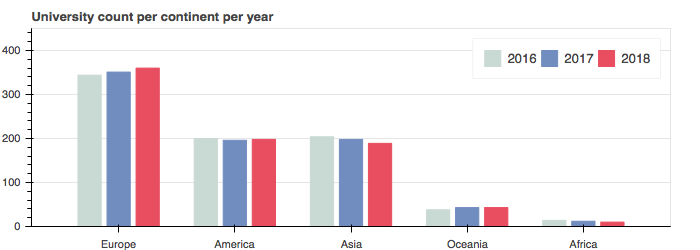
\includegraphics[scale=0.59]{images/count_uni_world.png}\\
\end{figure} 
Europa had driehonderd-vierenveertig studenten in 2016, driehonderd-eenenvijftig studenten in 2017 en driehonderd-zestig studenten in 2018, met een gemiddelde van driehonderd eenenvijftig, naar beneden afgerond, en een standaarddeviatie van zes. Amerika had tweehonderd universiteiten in de top achthonderd in 2016, honderd zesennegentig in 2017 en honderd achtennegentig in 2018. Dit levert een uiteindelijk gemiddelde op van honderd-achtennegentig, en een standaarddeviatie van 1. In Azië bevonden zich tweehonderd en vier universiteiten in de top achthonderd in 2016, honderd achtennegentig in 2017 en honderd negenentachtig in 2018. De gemiddelde hoeveelheid gerankte universiteiten was honderd zeven-en-negentig, met een standaarddeviatie van zes. Oceanië had achtendertig gerankte universiteiten in 2016 en drieënveertig universiteiten in zowel 2017 als 2018. Dit gaf een gemiddelde van eenenveertig universiteiten, met een standaarddeviatie van twee. Afrika had in 2016 veertien universiteiten in de ranglijst, twaalf in 2017 en tien universiteiten in 2018, voor een gemiddelde van twaalf universiteiten en een standaarddeviatie van een. 
\\
\\
De specifiekere verdeling per regio is weergegeven in de volgende tabellen. In Oceanië bevonden alle universiteiten zich echter in Australië en Nieuw-Zeeland, en vandaar ontbreekt deze tabel, aangezien deze geen informatie toevoegt.
\begin{center}
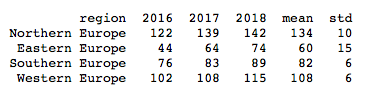
\includegraphics[scale=0.8]{images/data_euro.png}

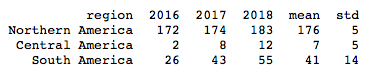
\includegraphics[scale=0.8]{images/data_amer.png}

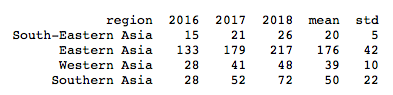
\includegraphics[scale=0.8]{images/data_asia.png}


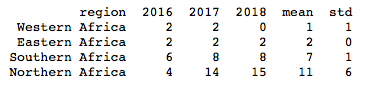
\includegraphics[scale=0.8]{images/data_afri.png}
\end{center}
Uit de data betreffende de internationale studenten is een licht negatief verband gevonden tussen het percentage interntionale studenten en de ranking van een universiteit. Vanuit een scatterplot is een \textit{best fit line} getrokken, wat een lineair verband opleverde. Met \textit{international ranking} als x-waarde en percentage interntaionale studenten als y-waarde is de lijn -0,0005x + 0,26 gevonden.\\

\begin{center}
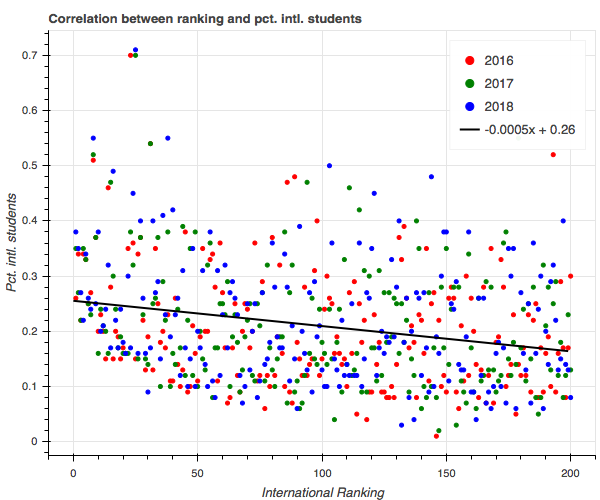
\includegraphics[scale=0.4]{images/pct_int_students.png}
\end{center}


Uit de data voor de verhouding tussen mannelijke en vrouwelijke studenten leverde geen duidelijk verband als resultaat gekomen. Wel kan er worden gezien dat er in de top tien universiteiten een hoger percentage mannelijke studenten bestaat. Ook is te zien dat het grootste deel van de uitschieters richting het mannelijke deel van de studenten slaat. 
\begin{figure}
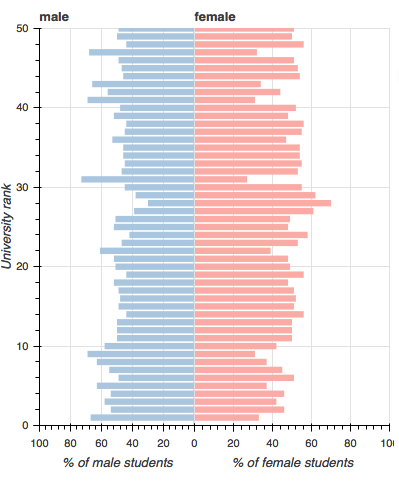
\includegraphics[scale=0.4]{images/male_female_2016.png}
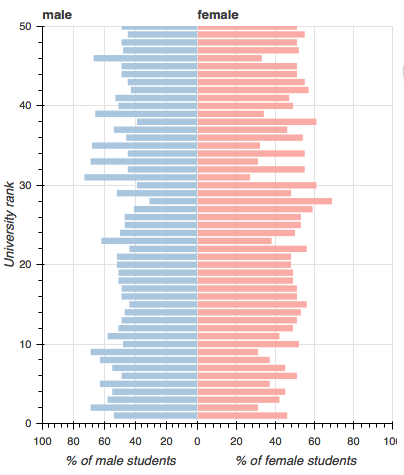
\includegraphics[scale=0.4]{images/male_female_2017.png}
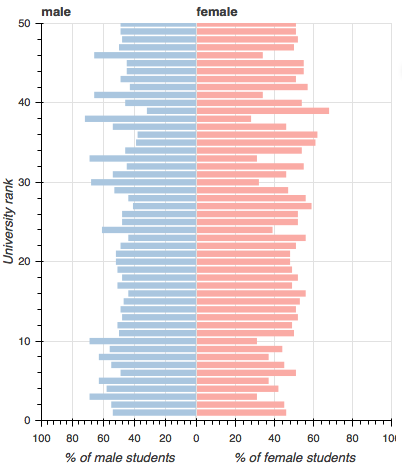
\includegraphics[scale=0.4]{images/male_female_2018.png}
\end{figure}
\newpage

De verdeling van de scores is als volgt voor de jaren 2016, 2017 en 2018 respectievelijk.

\begin{center}

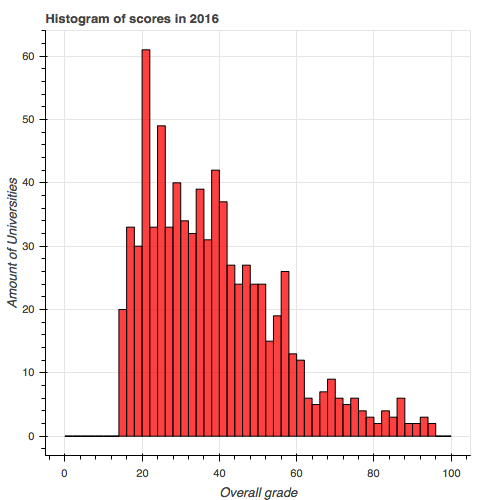
\includegraphics[scale=0.3]{images/scores_2016.png}

\end{center}
De gemiddelde score in 2016 is achtendertig komma zeven, de mediaan is vijfendertig komma zeven en een modus van twintig. Er zijn in 2016 geen scores lager dan veertien of hoger dan zesennegentig.  


\begin{center}
    
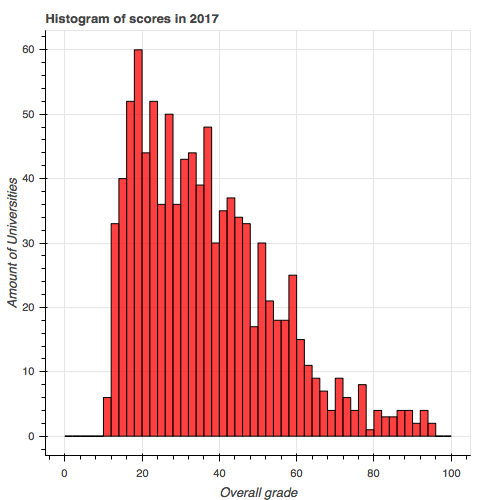
\includegraphics[scale=0.3]{images/scores_2017.png}

    
\end{center}

In 2017 is de gemiddelde score van de universiteiten zesendertig komma zeven, met een mediaan van drieëndertig komma zeven. De modus is zevenendertig, en er zijn geen scores lager dan tien of hoger dan zesennegentig.
\begin{center}

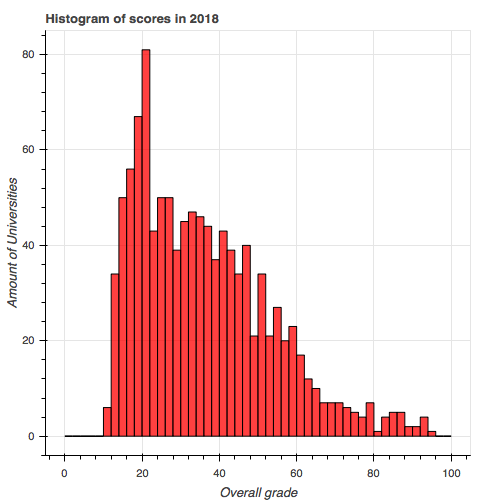
\includegraphics[scale=0.3]{images/scores_2018.png}

\end{center}

De universteiten scoorden gemiddeld zesendertig komma twee in 2018. De mediaan is drieendertig komma vier, en de modus is twintig. In 2018 zijn er geen scores lager dan tien of hoger dan zesennegentig gegeven. 

\begin{center}
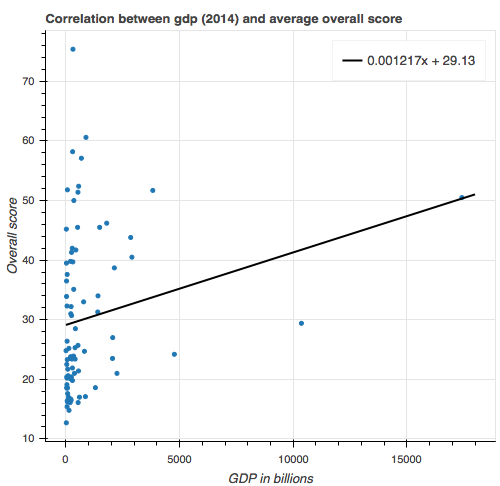
\includegraphics[scale=1]{images/gdp_score.png}
\end{center}

In de scatterplot waar het BNP tegenover verschillende gekozen maatstaven, waaronder ranking, \textit{overall score}, \textit{citation score}, \textit{industry score}, \textit{international outlook score}, \textit{research score} en \textit{teaching score}/. Met het BNP op de x-as en de gekozen maatstaaf op de y-as, is er gevonden dat er een positiefe relatie bestaat tussen het BNP en bijna alle maatstaven, er bestond alleen een negatiefe relatie tussen het BNP en de maatstaf, \textit{international outlook score}. Deze had een coefficient van -0.003. De maatstaaf die het sterkst positief was is de \textit{research score}.


\newpage
%-------------------------------------------------------------------------------
%	DISCUSSIE
%-------------------------------------------------------------------------------

\section*{Discussie}

Vanuit de diagrammen van de hoeveelheid universiteiten per continent en per regio zijn wat
opvallende trends op te merken. Zo is te zien dat er alleen in Europa (4.65\%) en Oceanië (13.2\%) de
afgelopen drie jaar een stijging in het aantal universiteiten op de ranglijst is. Dit laat zien dat in deze gebieden de kwaliteit van de universiteit genoeg is gestegen om die van de andere regio's uit de lijst te duwen, Daarentegen daalt de hoeveelheid universiteiten in Azië (-7.25\%), specifiek in Oost-Azië (-12.03\%). Het minst verandering is te zien in Amerika, waar de hoeveelheid universiteiten slechts daalt met 2 procent, hetgeen het de meest consistente regio maakt. Oost-Azië en Oceanië blijken de minst consistente regio's.

In de top tweehonderd universiteiten zijn helaas weinig verschillende aspecten te zien. Het percentage
internationale studenten verschilt weinig, tenzij er naar de volledige ranglijst wordt gekeken, er zijn dan in de top tweehonderd aanzienlijk meer internationale studenten dan bij de universiteiten die een lagere rank hebben. Als er gekeken wordt naar de lineaire benadering dan is er te zien dat er slechts een coëfficiënt van 0,005 is, wat dit beaamt. Dit kan zijn omdat er maar een kleine hoeveelheid studenten is die de mogelijk heeft internationaal te studeren, of vanwege het gebrek aan verschaffing van internationale studies aan deze universiteiten. Ook is het vanzelfsprekend dat de studenten die wel de mogelijkheid hebben om internationaal te studeren dit zullen doen aan de best mogelijke universiteit die voor hen beschikbaar is. In de verdeling tussen man en vrouw is helaas weinig opvallends te zien. De algemene verdeling tussen mannen en vrouwen lijkt overal in de buurt van éém op één te komen. Wel valt op dat in de top tien universiteiten er een meerderheid aan mannen studeert. Ook lijken de uitschieters vaker in de richting van de mannelijke studenten te wijzen.

Wat betreft andere opvallende verbanden, blijkt dat de scores van de universiteiten absoluut niet volgens een normale verdeling verspreid zijn. In elk jaar ligt het gemiddelde verassend laag met achtendertig komma zeven, zesendertig komma zeven en zesendertig komma twee in 2016, 2017 en 2018 respectievelijk. Ook is te zien dat de radar plots van de top vijf universiteiten per jaar behoorlijk overeenkomen in vorm. Een universiteit met een schijnbaar lage score kan zo toch bovengemiddeld blijken, en te top, met scores tot zesennegentig, blijkt ver boven de rest uit te steken. Ook de mmediaan blijkt per jaar lager te worden,va n vijfendertig komma zeven naar drieëndertig komma zeven en tenslotte drieëndertig komma vier. De modus valt op door niet te zakken, maar zelfs te stijgen in 2017 van twintig naar zevenendertig, om weer terug te zakken naar twintig in 2018.  

Daarnaast is er ook het Bruto Nationaal Product (BNP oftewel GDP) met de gemiddelde ranking en scores van universiteiten per land vergeleken. De Verenigde Staten en China zijn hier niet in meegenomen in de grafiek om dat dit \textit{outliers} waren omdat het BNP van deze landen zo groot is. Deze plot laat zien dat het BNP over het algemeen een positief relatie heeft op de ranking en scores van de universiteiten in een land. Hoe hoger het BNP is, hoe hoger ook de ranking en scores van de universiteiten zijn.

Er zijn uiteindelijk geen sterke verbanden gevonden tussen de verschillende aspecten van een universiteit en de uiteindelijke score die deze ontvangt. Een universiteit met een hogere score zal uiteindelijk een hoger percentage internationale studenten hebben, ook al blijkt dit verschil gering. De hoeveelheid mannen en vrouwen blijkt gemiddeld vrijwel gelijk te zijn, met een lichte voorkeur naar mannelijke studenten. 
De hypothese is dan ook weerlegd, en er zijn geen factoren die een directe invloed uitoefenen die groot genoeg is om een impact te hebben op de uiteindelijke score van een universiteit


\newpage

%-------------------------------------------------------------------------------
%	REFERENTIES
%-------------------------------------------------------------------------------


\begin{thebibliography}{9}
\bibitem{Times} 
Times Higher Education. \textit{World University Rankings 2016, 2017 \& 2018}. \url{https://www.timeshighereducation.com/world-university-rankings/2018/world-ranking#!/page/0/length/25/sort_by/rank/sort_order/asc/cols/stats.} (geraadpleegd 28 juni 2018)

\bibitem{CIA}
Central Intelligence Agency. \textit{The World Factbook (2014)}. \url{https://www.cia.gov/library/publications/the-world-factbook/fields/2195.html}\\ (geraadpleegd 28 juni 2018)

\bibitem{Bokeh}
Bokeh. \url{https://bokeh.pydata.org/en/latest/} (geraadpleegd op 28 juni 2018)

\bibitem{Plotly}
Plotly. \textit{Choropleth Maps in Python}. \url{https://plot.ly/python/choropleth-maps/}\\ (geraadpleegd op 28 juni 2018)

\end{thebibliography}

\section*{Appendix}

De machine learning code in fill.py:
\begin{lstlisting}

import numpy as np
from sklearn.linear_model import LinearRegression
from sklearn.model_selection import train_test_split


def male_female_fill(df):

    # converts all missing datapoints in column male into
    # mean of same country
    df.loc[df.male.isnull(), 'male'] = (df.groupby('country')
                                        .male.transform('mean'))
    # converts type to integer
    df.male = df.male.astype(int)
    # calculates female percentage based on male percentage
    df['female'] = 100 - df['male']

    return df




def pct_intl_student_fill(df):

    # converts string representation to float representation
    df['pct_intl_student'] = (df['pct_intl_student'].str.replace(r'%', r'.0')
                              .astype('float') / 100.0)
    # fills missing data points with 0 value
    df['pct_intl_student'] = df['pct_intl_student'].fillna(0)

    return df


def score_industry_fill(df):

    # columns we will use for predicting score_industry
    coi = ['ranking',
           'score_overall',
           'score_teaching',
           'score_research',
           'score_citation',
           'score_int_outlook',
           ]

    # get all rows that do not miss any value in any column
    not_nans = df['score_industry'].notnull()
    df_notnans = df[not_nans]

    # features
    x = np.array(df_notnans[coi])
    # labels
    y = np.array(df_notnans['score_industry'])

    # splits rows into testing and training data
    x_train, x_test, y_train, y_test = train_test_split(x, y, test_size=0.25)

    # classifier that we use, Multiple Linear Regression
    clf = LinearRegression()
    # trains classifier on trainig data
    clf.fit(x_train, y_train)

    # prints amount of predicted values that are correct
    # compares with the testing data
    print("score_industry: ", clf.score(x_test, y_test))

    # fills in missing values with classifier predicted values
    df_nans = df.loc[~not_nans].copy()
    df_nans['score_industry'] = clf.predict(df_nans[coi])
    df.score_industry.fillna(df_nans.score_industry, inplace=True)
    df['score_industry'] = round(df['score_industry'], 2)

    return df


def score_overall_fill(df):

    # columns we will se for predicting score_overall
    coi = ['score_teaching',
           'score_research',
           'score_citation',
           'score_int_outlook',
           ]

    # gets all rows that are not missing any value in any column
    not_nans = df['score_overall'].notnull()
    df_not_nans = df[not_nans]

    # features
    x = np.array(df_not_nans[coi])
    # labels
    y = np.array(df_not_nans['score_overall'])
    # splits non empty rows into training and testing data
    x_train, x_test, y_train, y_test = train_test_split(x, y, test_size=0.25)

    # classifier that we use, Multiple Linear Regression
    clf = LinearRegression()
    # 
    clf.fit(x_train, y_train)
    print("score_overall: ", clf.score(x_test, y_test))
    df_nans = df.loc[~not_nans].copy()
    df_nans['score_overall'] = clf.predict(df_nans[coi])
    df.score_overall.fillna(df_nans.score_overall, inplace=True)
    df['score_overall'] = round(df['score_overall'], 2)

    return df


\end{lstlisting}
Ongebruikte plots en tabellen
\begin{center}
    

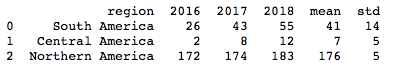
\includegraphics[scale=1]{images/data1.png}\\
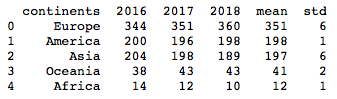
\includegraphics[scale=1]{images/data2.png}\\
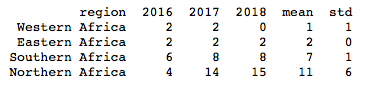
\includegraphics[scale=1]{images/data_afri.png}\\
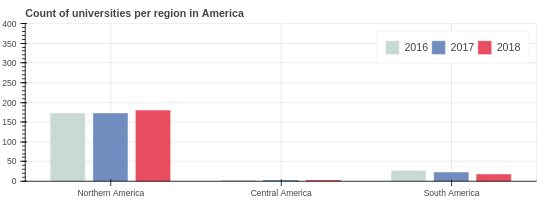
\includegraphics[scale=0.5]{images/count_uni_amer.png}\\
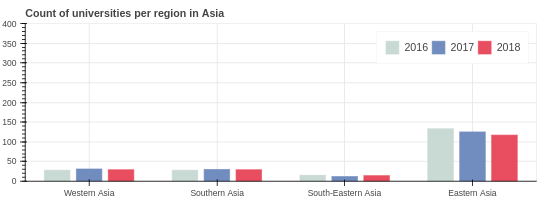
\includegraphics[scale=0.5]{images/count_uni_asia.png}\\
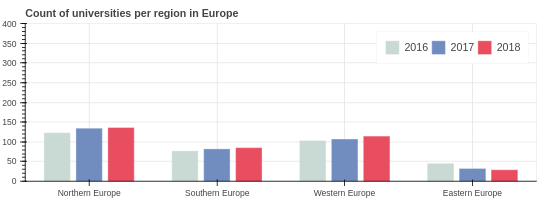
\includegraphics[scale=0.5]{images/count_uni_eur.png}\\
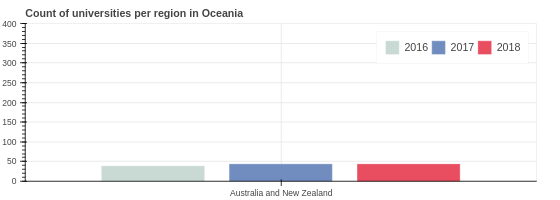
\includegraphics[scale=0.5]{images/count_uni_ocea.png}\\
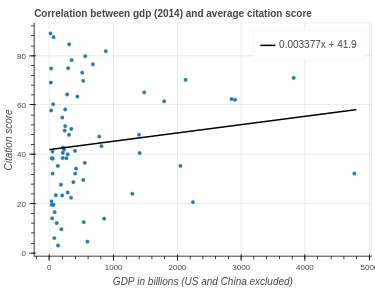
\includegraphics[scale=0.5]{images/gdp_citation.png}\\
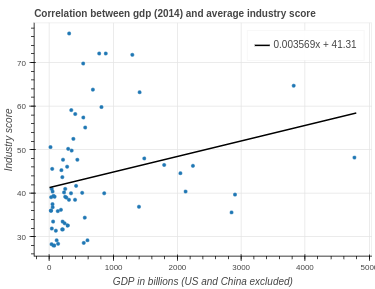
\includegraphics[scale=0.5]{images/gdp_industry.png}\\
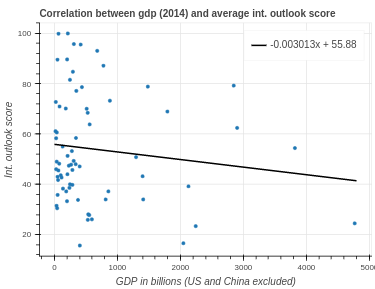
\includegraphics[scale=0.5]{images/gdp_outlook.png}\\
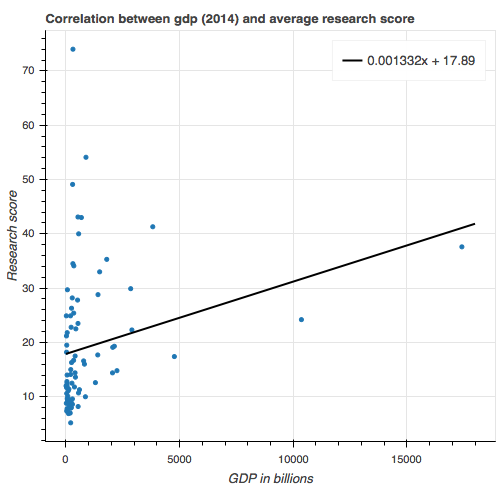
\includegraphics[scale=0.5]{images/gdp_research.png}\\
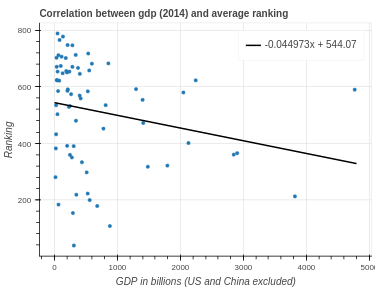
\includegraphics[scale=0.5]{images/gdp_ranking.png}\\
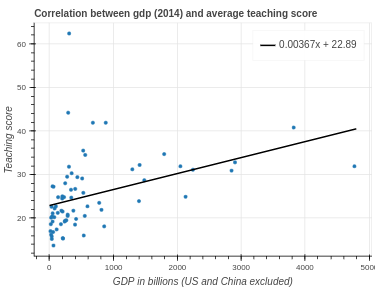
\includegraphics[scale=0.5]{images/gdp_teaching.png}\\
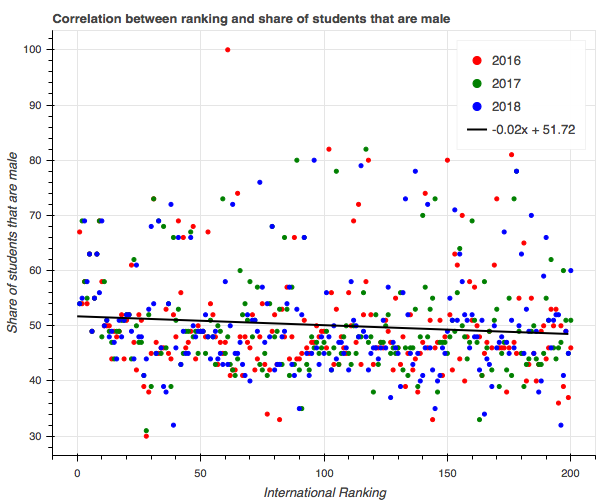
\includegraphics[scale=0.5]{images/male_students.png}\\
\includegraphics[scale=0.2]{images/radar2.png}\\
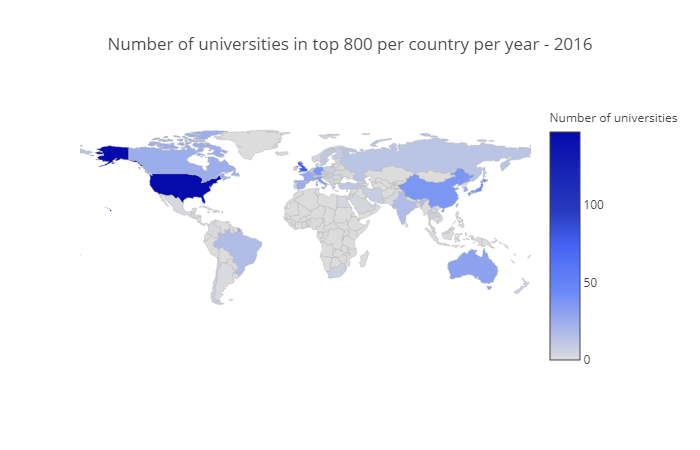
\includegraphics[scale=0.5]{images/worldmap_2016.png}\\
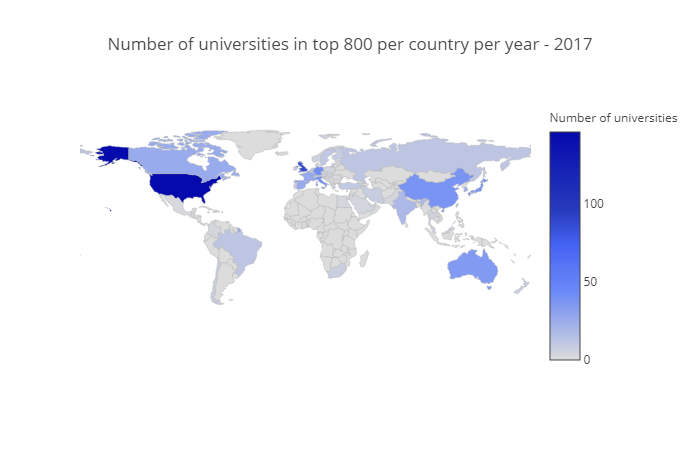
\includegraphics[scale=0.5]{images/worldmap_2017.png}\\
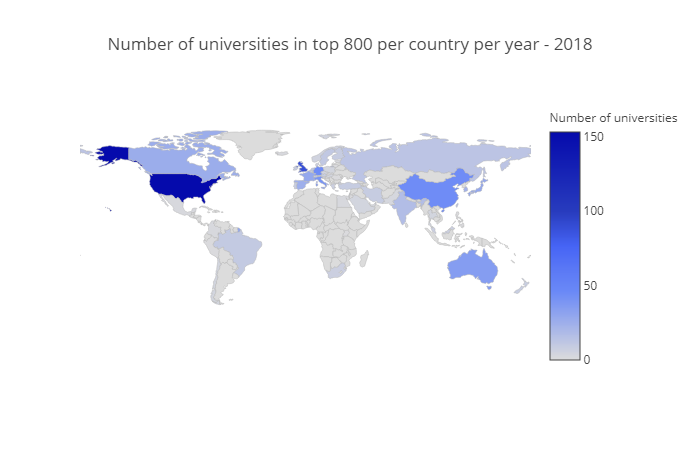
\includegraphics[scale=0.5]{images/worldmap_2018.png}\\
\end{center}

Alle overige code is te vinden op de GitHub pagina DanielPerezJensen/bscKI-data-analyse:     \url{https://github.com/DanielPerezJensen/bscKI-data-analyse}







%-------------------------------------------------------------------------------
%	BIJLAGEN EN EINDE
%-------------------------------------------------------------------------------

%\section{Bijlage A}
%\section{Bijlage B}
%\section{Bijlage C}
\end{document}
